\chapter{लुइस संरचनाएँ और अणुओं की आकृति}\label{ch:g10:lewis-and-shape}

कार्बन डाइऑक्साइड का \omterm{def:g7:atoms-and-molecules:molecule}{अणु} सीधा है; पानी का \omterm{def:g7:atoms-and-molecules:molecule}{अणु} मुड़ा हुआ। आकृति का यही एक अंतर
उन कारणों में से एक है जिनसे पानी, जिसके \omterm{def:g7:atoms-and-molecules:molecule}{अणु} कार्बन डाइऑक्साइड के \omterm{def:g7:atoms-and-molecules:molecule}{अणुओं} से हल्के
हैं, कमरे के ताप पर द्रव है जबकि कार्बन डाइऑक्साइड गैस। \omterm{def:g7:atoms-and-molecules:molecule}{अणु} में \omterm{def:g7:atoms-and-molecules:atom}{परमाणु} साझा
\omterm{def:g9:inside-the-atom:nucleus}{इलेक्ट्रॉनों} से जुड़े रहते हैं, और \omterm{def:g9:inside-the-atom:nucleus}{इलेक्ट्रॉन} जिस ढंग से साझा होते हैं, वही आकृति
तय करता है। यह अध्याय साझा \omterm{def:g9:inside-the-atom:nucleus}{इलेक्ट्रॉनों} को बनाता है, और उनसे आकृति का
अनुमान लगाता है।

\begin{recall}
\omterm{def:g10:electron-shells:valence}{संयोजकता इलेक्ट्रॉन} बाहरी \omterm{def:g10:electron-shells:configuration}{कोश} के \omterm{def:g9:inside-the-atom:nucleus}{इलेक्ट्रॉन} हैं; \omterm{def:g7:atoms-and-molecules:atom}{परमाणु} किसी \omterm{def:g10:electron-shells:family}{उत्कृष्ट गैस} का
विन्यास पाने की प्रवृत्ति रखते हैं: बाहरी \omterm{def:g10:electron-shells:configuration}{कोश} में आठ \omterm{def:g9:inside-the-atom:nucleus}{इलेक्ट्रॉन} (\omterm{def:g10:electron-shells:octet}{अष्टक नियम}),
या हाइड्रोजन के लिए दो (\omterm{def:g10:electron-shells:octet}{द्विक नियम})
(\cref{ch:g10:electron-shells})। आण्विक मॉडल \omterm{def:g7:atoms-and-molecules:atom}{परमाणुओं} को गेंदों और
आबंधों को छड़ों के रूप में दिखाते हैं (\cref{ch:g7:atoms-and-molecules})।
\end{recall}

\section{सहसंयोजी आबंध}

\begin{definition}[सहसंयोजी आबंध]\label{def:g10:lewis-and-shape:covalent-bond}
\emph{सहसंयोजी आबंध}\index{सहसंयोजी आबंध} दो \omterm{def:g7:atoms-and-molecules:atom}{परमाणुओं} द्वारा साझा किया गया
\omterm{def:g9:inside-the-atom:nucleus}{इलेक्ट्रॉनों} का एक युग्म है; आम तौर पर हर \omterm{def:g7:atoms-and-molecules:atom}{परमाणु} युग्म का एक \omterm{def:g9:inside-the-atom:nucleus}{इलेक्ट्रॉन} देता है।
दोनों \omterm{def:g7:atoms-and-molecules:atom}{परमाणु} साझा युग्म को अपने बाहरी \omterm{def:g10:electron-shells:configuration}{कोश} में गिनते हैं, जिससे दोनों द्विक या
अष्टक पा लेते हैं।
\end{definition}

\begin{definition}[आबंधी युग्म और एकाकी युग्म]\label{def:g10:lewis-and-shape:lone-pair}
\omterm{def:g7:atoms-and-molecules:molecule}{अणु} में हर \omterm{def:g7:atoms-and-molecules:atom}{परमाणु} के \omterm{def:g10:electron-shells:valence}{संयोजकता इलेक्ट्रॉन} युग्मों में बँटे होते हैं।
\emph{आबंधी युग्म}\index{आबंधी युग्म} दो \omterm{def:g7:atoms-and-molecules:atom}{परमाणुओं} के बीच साझा होता है और
एक \omterm{def:g10:lewis-and-shape:covalent-bond}{सहसंयोजी आबंध} बनाता है; \emph{एकाकी युग्म}\index{एकाकी युग्म} एक ही \omterm{def:g7:atoms-and-molecules:atom}{परमाणु}
का होता है और किसी आबंध में भाग नहीं लेता।
\end{definition}

\begin{proposition}[परमाणु कितने आबंध बनाता है]\label{prop:g10:lewis-and-shape:valence}
\omterm{def:g7:atoms-and-molecules:atom}{परमाणु} उतने \omterm{def:g10:lewis-and-shape:covalent-bond}{सहसंयोजी आबंध} बनाता है जितने \omterm{def:g9:inside-the-atom:nucleus}{इलेक्ट्रॉनों} की उसे अपना द्विक या
अष्टक पूरा करने के लिए कमी है:
\begin{center}
\small
\begin{tabular}{lcccc}
\hline
\omterm{def:g7:atoms-and-molecules:atom}{परमाणु} & \omterm{def:g10:electron-shells:valence}{संयोजकता इलेक्ट्रॉन} & आबंध & \omterm{def:g10:lewis-and-shape:lone-pair}{एकाकी युग्म} & उदाहरण \\
\hline
H & 1 & 1 & 0 & \ce{H2} \\
C & 4 & 4 & 0 & \ce{CH4} \\
N & 5 & 3 & 1 & \ce{NH3} \\
O & 6 & 2 & 2 & \ce{H2O} \\
Cl & 7 & 1 & 3 & \ce{HCl} \\
\hline
\end{tabular}
\end{center}
\end{proposition}

\section{लुइस संरचनाएँ}

\begin{definition}[लुइस संरचना]\label{def:g10:lewis-and-shape:lewis-structure}
किसी \omterm{def:g7:atoms-and-molecules:molecule}{अणु} की \emph{लुइस संरचना}\index{लुइस संरचना} उसके \omterm{def:g7:atoms-and-molecules:atom}{परमाणुओं} को उनके
प्रतीकों से, हर \omterm{def:g10:lewis-and-shape:lone-pair}{आबंधी युग्म} को दो \omterm{def:g7:atoms-and-molecules:atom}{परमाणुओं} के बीच एक रेखा से, और हर \omterm{def:g10:lewis-and-shape:lone-pair}{एकाकी
युग्म} को उसके \omterm{def:g7:atoms-and-molecules:atom}{परमाणु} के पास दो बिंदुओं से दिखाती है।
\end{definition}

\begin{definition}[द्विआबंध और त्रिआबंध]\label{def:g10:lewis-and-shape:multiple-bond}
दो \omterm{def:g7:atoms-and-molecules:atom}{परमाणु} \omterm{def:g9:inside-the-atom:nucleus}{इलेक्ट्रॉनों} के दो युग्म साझा कर सकते हैं, जो \emph{द्विआबंध}\index{द्विआबंध}
है और दो रेखाओं से बनाया जाता है, या तीन युग्म, जो
\emph{त्रिआबंध}\index{त्रिआबंध} है और तीन रेखाओं से बनाया जाता है।
\end{definition}

\begin{method}[लुइस संरचना बनाना]\label{met:g10:lewis-and-shape:draw}
\begin{enumerate}
  \item सभी \omterm{def:g7:atoms-and-molecules:atom}{परमाणुओं} के \omterm{def:g10:electron-shells:valence}{संयोजकता इलेक्ट्रॉनों} को जोड़िए, और युग्मों की संख्या
        पाने के लिए आधा कीजिए।
  \item \omterm{def:g7:atoms-and-molecules:atom}{परमाणुओं} को एकल आबंधों से जोड़िए (एक आबंध बनाने वाली हाइड्रोजन
        हमेशा बाहर होती है; कार्बन आम तौर पर केंद्र में होता है)।
  \item बचे हुए युग्मों को \omterm{def:g10:lewis-and-shape:lone-pair}{एकाकी युग्मों} के रूप में रखिए, पहले बाहरी \omterm{def:g7:atoms-and-molecules:atom}{परमाणुओं}
        पर, ताकि उनके अष्टक पूरे हों।
  \item अगर किसी \omterm{def:g7:atoms-and-molecules:atom}{परमाणु} का अष्टक अब भी अधूरा है, तो किसी पड़ोसी के \omterm{def:g10:lewis-and-shape:lone-pair}{एकाकी युग्म}
        को दूसरे (या तीसरे) साझा युग्म में बदलिए।
  \item जाँचिए: हर हाइड्रोजन के पास 2 \omterm{def:g9:inside-the-atom:nucleus}{इलेक्ट्रॉन} हों, हर दूसरे \omterm{def:g7:atoms-and-molecules:atom}{परमाणु} के पास 8,
        और सारे युग्म इस्तेमाल हो चुके हों।
\end{enumerate}
\end{method}

\begin{example}[कार्बन डाइऑक्साइड]\label{ex:g10:lewis-and-shape:co2}
\ce{CO2}: $4 + 2 \times 6 = 16$ \omterm{def:g10:electron-shells:valence}{संयोजकता इलेक्ट्रॉन}, 8 युग्म। एकल आबंध
\ce{O-C-O} 2 युग्म लेते हैं; ऑक्सीजनों पर 6 \omterm{def:g10:lewis-and-shape:lone-pair}{एकाकी युग्म} उन्हें पूरा कर देते हैं,
पर तब कार्बन के पास केवल 4 \omterm{def:g9:inside-the-atom:nucleus}{इलेक्ट्रॉन} रहते हैं। हर ऑक्सीजन के एक \omterm{def:g10:lewis-and-shape:lone-pair}{एकाकी युग्म} को
साझा युग्म में बदलने से दो \omterm{def:g10:lewis-and-shape:multiple-bond}{द्विआबंध} बनते हैं: अब हर \omterm{def:g7:atoms-and-molecules:atom}{परमाणु} के पास अष्टक है।
\end{example}

\begin{omfigure}
\setchemfig{atom sep=2.0em}
\begin{tabular}{cccccc}
\chemfig{H-H} & \chemfig{H-\charge{0=\:,90=\:,270=\:}{Cl}} & \chemfig{H-\charge{90=\:,270=\:}{O}-H} &
\chemfig{H-\charge{90=\:}{N}(-[6]H)-H} & \chemfig{H-C(-[2]H)(-[6]H)-H} &
\chemfig{\charge{135=\:,225=\:}{O}=C=\charge{45=\:,315=\:}{O}} \\[4pt]
\small \ce{H2} & \small \ce{HCl} & \small \ce{H2O} & \small \ce{NH3} & \small \ce{CH4} & \small \ce{CO2} \\[10pt]
\chemfig{\charge{180=\:}{N}~\charge{0=\:}{N}} & \chemfig{\charge{135=\:,225=\:}{O}=\charge{45=\:,315=\:}{O}} &
\chemfig{C(-[3]H)(-[5]H)=C(-[1]H)-[7]H} & \chemfig{H-C~\charge{0=\:}{N}} &
\chemfig{H-C(-[6]H)=\charge{45=\:,315=\:}{O}} & \\[4pt]
\small \ce{N2} & \small \ce{O2} & \small \ce{C2H4} & \small \ce{HCN} & \small मेथेनैल \ce{CH2O} &
\end{tabular}

{\small ग्यारह \omterm{def:g7:atoms-and-molecules:molecule}{अणुओं} की \omterm{def:g10:lewis-and-shape:lewis-structure}{लुइस संरचनाएँ}। हाइड्रोजन को छोड़कर हर \omterm{def:g7:atoms-and-molecules:atom}{परमाणु} चार
युग्मों (आबंधों और \omterm{def:g10:lewis-and-shape:lone-pair}{एकाकी युग्मों}) से घिरा है: एक अष्टक।}
\end{omfigure}

\section{अणुओं की आकृति}

\begin{proposition}[इलेक्ट्रॉन युग्म एक-दूसरे से यथासंभव दूर रहते हैं]\label{prop:g10:lewis-and-shape:shape}
केंद्रीय \omterm{def:g7:atoms-and-molecules:atom}{परमाणु} के चारों ओर \omterm{def:g9:inside-the-atom:nucleus}{इलेक्ट्रॉनों} के समूह --- हर एकल, द्वि या
त्रि आबंध, और हर \omterm{def:g10:lewis-and-shape:lone-pair}{एकाकी युग्म} --- एक-दूसरे को प्रतिकर्षित करते हैं और यथासंभव दूर
जाकर टिकते हैं। इससे \omterm{def:g7:atoms-and-molecules:molecule}{अणु} की आकृति निकलती है:
\begin{center}
\small
\begin{tabular}{llll}
\hline
केंद्र के चारों ओर समूह & जिनमें \omterm{def:g10:lewis-and-shape:lone-pair}{एकाकी युग्म} & आकृति & उदाहरण \\
\hline
2 & 0 & रैखिक, कोण \ang{180} & \ce{CO2}, \ce{HCN} \\
3 & 0 & समतल त्रिकोण, कोण \ang{120} & \ce{CH2O}, \ce{C2H4} \\
4 & 0 & चतुष्फलक, कोण \ang{109.5} & \ce{CH4} \\
4 & 1 & पिरामिड & \ce{NH3} \\
4 & 2 & मुड़ी हुई & \ce{H2O} \\
\hline
\end{tabular}
\end{center}
\end{proposition}
\admitted

\begin{remark}[यह कहाँ से आता है]\label{rem:g10:lewis-and-shape:vsepr}
यह नियम एक मॉडल है, और छोटे \omterm{def:g7:atoms-and-molecules:molecule}{अणुओं} के लिए अद्भुत रूप से अच्छा काम करता है;
विश्वविद्यालय के प्रथम वर्ष के खंड में इसे सटीक बनाया गया है, और आंशिक रूप से समझाया
गया है। \omterm{def:g10:lewis-and-shape:lone-pair}{एकाकी युग्म} \omterm{def:g10:lewis-and-shape:lone-pair}{आबंधी युग्मों} से थोड़ी ज़्यादा जगह घेरते हैं: अमोनिया
(\ang{106.7}) और पानी (\ang{104.5}) का कोण मेथेन के
\ang{109.5} से थोड़ा छोटा है।
\end{remark}

\begin{omfigure}
\begin{tikzpicture}[font=\small]
  % methane, tetrahedral, in perspective
  \begin{scope}
    \node[aC] (c) at (0,0) {};
    \node[aH, minimum size=3.6mm] (hb) at (0.3,-0.12) {};
    \node[aH] (h1) at (0,1.05) {};
    \node[aH] (h2) at (-1.0,-0.45) {};
    \node[aH] (h3) at (0.72,-0.5) {};
    \begin{scope}[on background layer]
      \foreach \h in {h1,h2,h3,hb} \draw[bond] (c.center) -- (\h.center);
    \end{scope}
    \node[aC] at (0,0) {};
    \node at (0,-1.35) {मेथेन: चतुष्फलक};
    \node[font=\footnotesize] at (-0.55,0.55) {\ang{109.5}};
  \end{scope}
  % ammonia, pyramid
  \begin{scope}[xshift=4.2cm]
    \fill[omDef!25] (0,0.2) ellipse (0.18 and 0.45);
    \node[font=\scriptsize, omDef] at (0,1.0) {एकाकी युग्म};
    \node[aN] (n) at (0,0) {};
    \node[aH] (h1) at (-0.95,-0.5) {};
    \node[aH] (h2) at (0.7,-0.55) {};
    \node[aH, minimum size=3.6mm] (h3) at (0.25,-0.2) {};
    \begin{scope}[on background layer]
      \foreach \h in {h1,h2,h3} \draw[bond] (n.center) -- (\h.center);
    \end{scope}
    \node[aN] at (0,0) {};
    \node at (0,-1.35) {अमोनिया: पिरामिड};
  \end{scope}
  % water, bent
  \begin{scope}[xshift=8.4cm]
    \fill[omDef!25, rotate=25] (0,0.2) ellipse (0.16 and 0.42);
    \fill[omDef!25, rotate=-25] (0,0.2) ellipse (0.16 and 0.42);
    \node[aO] (o) at (0,0) {};
    \node[aH] (h1) at (-0.8,-0.58) {};
    \node[aH] (h2) at (0.8,-0.58) {};
    \begin{scope}[on background layer]
      \draw[bond] (o.center) -- (h1.center); \draw[bond] (o.center) -- (h2.center);
    \end{scope}
    \node[aO] at (0,0) {};
    \draw[black!60] (-0.32,-0.23) arc[start angle=216, end angle=324, radius=0.4];
    \node[font=\footnotesize] at (0,-0.65) {\ang{104.5}};
    \node at (0,-1.35) {पानी: मुड़ा हुआ};
  \end{scope}
  % carbon dioxide, linear
  \begin{scope}[xshift=12.0cm]
    \node[aO] (a) at (-0.8,0) {}; \node[aC] (c) at (0,0) {}; \node[aO] (b) at (0.8,0) {};
    \begin{scope}[on background layer]
      \foreach \d in {-1.6,1.6} {
        \draw[bond, line width=1.1pt] ([yshift=\d pt]a.center) -- ([yshift=\d pt]c.center);
        \draw[bond, line width=1.1pt] ([yshift=\d pt]c.center) -- ([yshift=\d pt]b.center);}
    \end{scope}
    \node at (0,-1.35) {कार्बन डाइऑक्साइड: रैखिक};
  \end{scope}
\end{tikzpicture}

{\small चार \omterm{def:g7:atoms-and-molecules:molecule}{अणुओं} की आकृतियाँ (\omterm{def:g10:lewis-and-shape:lone-pair}{एकाकी युग्म} छायांकित पालियों के रूप में)।
% ledger: ang:H2O, ang:NH3
मेथेन चतुष्फलक है, अमोनिया पिरामिड, पानी मुड़ा हुआ, कार्बन डाइऑक्साइड
सीधा।}
\end{omfigure}

\begin{omfigure}
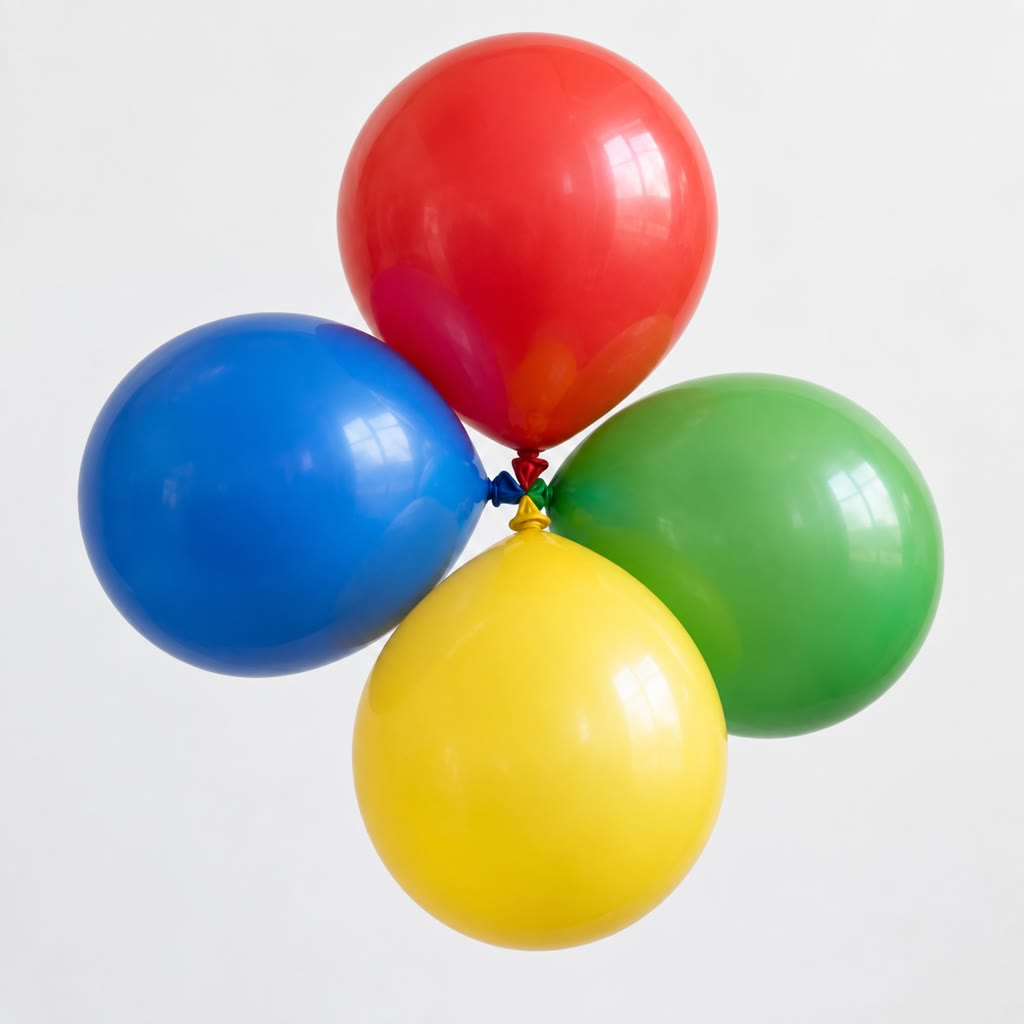
\includegraphics[width=0.38\linewidth]{images/book1/ai/g10-balloons-tetrahedron.jpg}

{\small आपस में बँधे चार गुब्बारे एक-दूसरे को यथासंभव दूर धकेलते हैं;
त्रिविम में वे एक चतुष्फलक के कोनों की ओर इशारा करते हैं, ठीक कार्बन \omterm{def:g7:atoms-and-molecules:atom}{परमाणु} के
चारों ओर के चार \omterm{def:g9:inside-the-atom:nucleus}{इलेक्ट्रॉन} युग्मों की तरह।}
\end{omfigure}

\section{अणुओं को त्रिविम रूप में बनाना}

\begin{notation}[फन्नियाँ और डैश]\label{not:g10:lewis-and-shape:wedge}
किसी \omterm{def:g7:atoms-and-molecules:molecule}{अणु} को त्रिविम रूप में सपाट कागज़ पर बनाने के लिए, कागज़ के तल में स्थित आबंध
एक सादी रेखा होता है, पाठक की ओर इशारा करता आबंध एक ठोस फन्नी,
और दूर की ओर इशारा करता आबंध एक डैश वाली फन्नी। तब मेथेन नीचे की तरह बनाया
जाता है: दो आबंध तल में, एक पाठक की ओर और एक पाठक से दूर।
\begin{center}
\chemfig{C(-[2]H)(-[4]H)(<[7]H)(<:[5]H)}
\end{center}
\end{notation}

\section{अभ्यास}

\begin{exercise}[$\star$]\label{exo:g10:lewis-and-shape:1}
\omterm{def:g10:lewis-and-shape:covalent-bond}{सहसंयोजी आबंध} क्या है? \omterm{def:g10:lewis-and-shape:lone-pair}{एकाकी युग्म} क्या है?
\end{exercise}

\begin{exercise}[$\star$]\label{exo:g10:lewis-and-shape:2}
हाइड्रोजन, कार्बन, नाइट्रोजन और ऑक्सीजन आम तौर पर कितने \omterm{def:g10:lewis-and-shape:covalent-bond}{सहसंयोजी आबंध}
बनाते हैं? अष्टक और द्विक नियमों से समझाइए।
\end{exercise}

\begin{exercise}[$\star$]\label{exo:g10:lewis-and-shape:3}
हाइड्रोजन क्लोराइड, \ce{HCl}, की \omterm{def:g10:lewis-and-shape:lewis-structure}{लुइस संरचना} बनाइए, और क्लोरीन के चारों ओर
के \omterm{def:g9:inside-the-atom:nucleus}{इलेक्ट्रॉन} गिनिए।
\end{exercise}

\begin{exercise}[$\star$]\label{exo:g10:lewis-and-shape:4}
\omterm{def:g7:atoms-and-molecules:molecule}{अणु} \ce{NH3} में कुल कितने \omterm{def:g10:electron-shells:valence}{संयोजकता इलेक्ट्रॉन} हैं? कितने
युग्म?
\end{exercise}

\begin{exercise}[$\star$]\label{exo:g10:lewis-and-shape:5}
\ce{CH4}, \ce{NH3}, \ce{H2O} और \ce{CO2} की आकृतियाँ बताइए।
\end{exercise}

\begin{exercise}[$\star\star$]\label{exo:g10:lewis-and-shape:6}
हाइड्रोजन सल्फ़ाइड, \ce{H2S}, की \omterm{def:g10:lewis-and-shape:lewis-structure}{लुइस संरचना} बनाइए (सल्फ़र ऑक्सीजन वाले
समूह में है), और उसकी आकृति का अनुमान लगाइए।
\end{exercise}

\begin{exercise}[$\star\star$]\label{exo:g10:lewis-and-shape:7}
विधि का चरण-दर-चरण पालन करते हुए नाइट्रोजन, \ce{N2}, की \omterm{def:g10:lewis-and-shape:lewis-structure}{लुइस संरचना}
बनाइए।
\end{exercise}

\begin{exercise}[$\star\star$]\label{exo:g10:lewis-and-shape:8}
मेथेनॉल, \ce{CH3OH}, की \omterm{def:g10:lewis-and-shape:lewis-structure}{लुइस संरचना} बनाइए, और कार्बन के चारों ओर तथा
ऑक्सीजन के चारों ओर की आकृति बताइए।
\end{exercise}

\begin{exercise}[$\star\star$]\label{exo:g10:lewis-and-shape:9}
\ce{CO2} रैखिक और \ce{H2O} मुड़ा हुआ क्यों है, हालाँकि दोनों में एक केंद्रीय \omterm{def:g7:atoms-and-molecules:atom}{परमाणु}
दो दूसरों से जुड़ा है?
\end{exercise}

\begin{exercise}[$\star\star$]\label{exo:g10:lewis-and-shape:10}
एथीन, \ce{C2H4}, की \omterm{def:g10:lewis-and-shape:lewis-structure}{लुइस संरचना} बनाइए, और हर कार्बन \omterm{def:g7:atoms-and-molecules:atom}{परमाणु} के चारों ओर की
आकृति बताइए।
\end{exercise}

\begin{exercise}[$\star\star$]\label{exo:g10:lewis-and-shape:11}
टेट्राक्लोरोमेथेन, \ce{CCl4}, की \omterm{def:g10:lewis-and-shape:lewis-structure}{लुइस संरचना} बनाइए, और उसकी आकृति का
अनुमान लगाइए।
\end{exercise}

\begin{exercise}[$\star\star\star$]\label{exo:g10:lewis-and-shape:12}
दो \omterm{def:g7:atoms-and-molecules:molecule}{अणुओं} का सूत्र \ce{C2H6O} है। हर एक के लिए एक \omterm{def:g10:lewis-and-shape:lewis-structure}{लुइस संरचना} बनाइए
(एक में O--H आबंध है, दूसरे में C--O--C श्रृंखला)।
\end{exercise}

\begin{exercise}[$\star\star\star$]\label{exo:g10:lewis-and-shape:13}
\omterm{def:g10:lewis-and-shape:lone-pair}{एकाकी युग्मों} की मदद से समझाइए कि अमोनिया का कोण (\ang{106.7}) मेथेन
(\ang{109.5}) से छोटा क्यों है, और पानी का (\ang{104.5}) उससे भी
छोटा क्यों।
\end{exercise}

\begin{exercise}[$\star\star\star$]\label{exo:g10:lewis-and-shape:14}
हाइड्रोजन सायनाइड, \ce{HCN}, और मेथेनैल,
\ce{CH2O}, की \omterm{def:g10:lewis-and-shape:lewis-structure}{लुइस संरचनाएँ} बनाइए, और उनकी आकृतियाँ बताइए।
\end{exercise}

\begin{exercise}[$\star\star\star$]\label{exo:g10:lewis-and-shape:15}
ओज़ोन, \ce{O3}, तीन ऑक्सीजन \omterm{def:g7:atoms-and-molecules:atom}{परमाणुओं} की एक श्रृंखला है। उसके संयोजकता युग्म गिनिए
और ऐसी \omterm{def:g10:lewis-and-shape:lewis-structure}{लुइस संरचना} बनाइए जिसमें हर ऑक्सीजन के पास अष्टक हो (एक
\omterm{def:g10:lewis-and-shape:multiple-bond}{द्विआबंध}, एक एकल आबंध)। अनुमान लगाइए कि \omterm{def:g7:atoms-and-molecules:molecule}{अणु} रैखिक है या
मुड़ा हुआ।
\end{exercise}

\section{समस्या: घन के भीतर एक अणु}

\begin{problem}[{सप्ताहांत समस्या --- आण्विक मॉडल किट की कार्बन गेंदों की
रूपरेखा: छेद किस कोण पर किए जाएँ?}]
\label{pb:g10:lewis-and-shape:1}
% ledger: ang:H2O, ang:NH3
एक कंपनी आण्विक मॉडल किट बनाती है। काली कार्बन गेंदों में चार छेद होने चाहिए,
ताकि मेथेन, एथेन और कार्बन के दूसरे \omterm{def:g7:atoms-and-molecules:molecule}{अणु} सही आकृति में
बनें। इंजीनियर एक युक्ति अपनाता है: एक समचतुष्फलक एक घन के भीतर
समा जाता है, उसके चार कोने घन के चार कोनों पर होते हैं, और कोई भी दो एक ही
किनारे पर नहीं होते।

\medskip
\noindent\textbf{भाग I --- \omterm{def:g10:lewis-and-shape:lewis-structure}{लुइस संरचनाएँ}।}
\begin{enumerate}
  \item मेथेन \ce{CH4}, अमोनिया \ce{NH3} और पानी \ce{H2O} की \omterm{def:g10:lewis-and-shape:lewis-structure}{लुइस
        संरचनाएँ} बनाइए।
  \item हर एक में केंद्रीय \omterm{def:g7:atoms-and-molecules:atom}{परमाणु} के चारों ओर \omterm{def:g9:inside-the-atom:nucleus}{इलेक्ट्रॉनों} के कितने समूह हैं?
  \item उनमें से कितने \omterm{def:g10:lewis-and-shape:lone-pair}{एकाकी युग्म} हैं?
  \item कार्बन गेंद को चार छेदों की ज़रूरत क्यों है, और (पानी के लिए) ऑक्सीजन
        गेंद को केवल दो की?
  \item एथेन, \ce{C2H6}, के मॉडल में दो कार्बन गेंदें लगती हैं। उसकी \omterm{def:g10:lewis-and-shape:lewis-structure}{लुइस
        संरचना} बनाइए। दोनों कार्बन गेंदों को कितनी छड़ें जोड़ती हैं, और कितनी
        हाइड्रोजन गेंदें चाहिए?
\end{enumerate}

\medskip
\noindent\textbf{भाग II --- आकृतियाँ।}
\begin{enumerate}[resume]
  \item तीनों \omterm{def:g7:atoms-and-molecules:molecule}{अणुओं} में से हर एक की आकृति बताइए।
  \item मापे गए कोण अमोनिया में \ang{106.7} और पानी में \ang{104.5} हैं।
        समझाइए कि ये मेथेन के कोण से छोटे क्यों हैं।
  \item अगर किट को सही कोण दिखाना है, तो पानी के लिए ऑक्सीजन गेंद केवल दो
        छेद ख़ाली छोड़ी गई कार्बन गेंद क्यों नहीं हो सकती?
  \item कार्बन डाइऑक्साइड में कार्बन \omterm{def:g7:atoms-and-molecules:atom}{परमाणु} दो \omterm{def:g10:lewis-and-shape:multiple-bond}{द्विआबंध} बनाता है। मॉडल में उनके
        बीच कौन-सा कोण होना चाहिए?
\end{enumerate}

\medskip
\noindent\textbf{भाग III --- घन।}
भुजा $a$ वाला एक घन लीजिए। कार्बन \omterm{def:g7:atoms-and-molecules:atom}{परमाणु} उसके केंद्र पर है; चारों
हाइड्रोजन \omterm{def:g7:atoms-and-molecules:atom}{परमाणु} घन के चार कोनों पर हैं, कोई भी दो एक ही किनारे पर नहीं।
\begin{enumerate}[resume]
  \item दिखाइए कि इनमें से कोई भी दो हाइड्रोजन \omterm{def:g7:atoms-and-molecules:atom}{परमाणु} घन के किसी फलक के
        विकर्ण के दोनों सिरों पर हैं। पाइथागोरस प्रमेय की मदद से उनके बीच की दूरी
        $a$ के पदों में निकालिए।
  \item पूरे घन का विकर्ण (एक कोने से सामने के कोने तक) $a\sqrt{3}$ लंबा है।
        कार्बन \omterm{def:g7:atoms-and-molecules:atom}{परमाणु} से हाइड्रोजन \omterm{def:g7:atoms-and-molecules:atom}{परमाणु} तक की दूरी
        निकालिए।
  \item किसी मॉडल में $a = \qty{1}{cm}$ लीजिए: दोनों दूरियाँ दो दशमलव स्थानों तक
        सेंटीमीटर में बताइए।
  \item चारों C--H दूरियाँ बराबर क्यों हैं?
\end{enumerate}

\medskip
\noindent\textbf{भाग IV --- कोण।}
कार्बन \omterm{def:g7:atoms-and-molecules:atom}{परमाणु} C और दो हाइड्रोजन \omterm{def:g7:atoms-and-molecules:atom}{परमाणु} H$_1$, H$_2$ एक समद्विबाहु
त्रिभुज बनाते हैं। मान लीजिए M, H$_1$H$_2$ का मध्यबिंदु है।
\begin{enumerate}[resume]
  \item समझाइए कि त्रिभुज C\,M\,H$_1$ में M पर समकोण क्यों है।
  \item इस समकोण त्रिभुज में कोण
        $\widehat{\text{M\,C\,H}_1}$ की ज्या निकालिए, जो कोण H--C--H का आधा है।
  \item अर्धकोण निकालिए, फिर कोण H--C--H, एक दशमलव
        स्थान तक।
  \item इस अध्याय की सारणी वाले कोण से तुलना कीजिए।
  \item बताइए कि कार्बन गेंद के छेद किस कोण पर किए
        जाने चाहिए।
\end{enumerate}
\end{problem}
